% sin関数のテイラー展開による近似比較図

\begin{figure}[H]
  \centering
  \caption{$f(x) = \sin(x)$のテイラー展開（3次多項式）}
  \label{fig:sin-taylor-first}
  \vspace{5pt}
  \begin{minipage}[b]{0.48\linewidth}
    \centering
    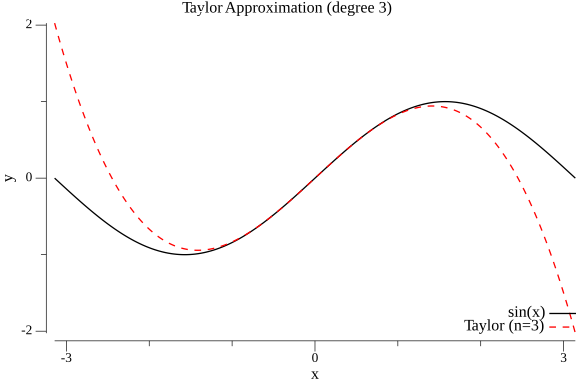
\includegraphics[width=1.0\linewidth]{material/sin/taylor/sin_taylor_n01.png}
  \end{minipage}
  \hfill
  \begin{minipage}[b]{0.48\linewidth}
    \centering
    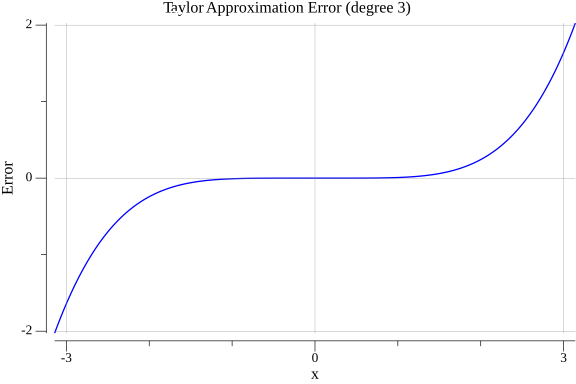
\includegraphics[width=1.0\linewidth]{material/sin/taylor/sin_taylor_err_n01.png}
  \end{minipage}
\end{figure}

\begin{figure}[H]
  \centering
  \caption{$f(x) = \sin(x)$のテイラー展開（11次多項式）}
  \label{fig:sin-taylor-2}
  \vspace{5pt}
  \begin{minipage}[b]{0.48\linewidth}
    \centering
    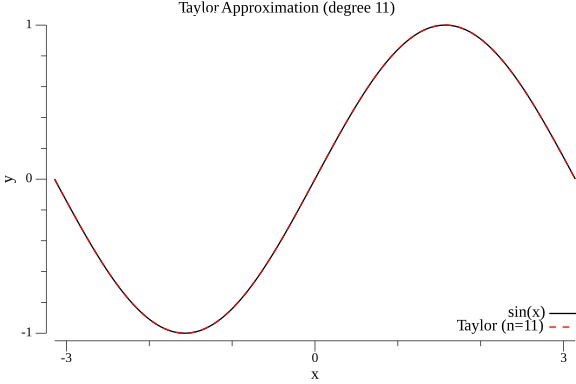
\includegraphics[width=1.0\linewidth]{material/sin/taylor/sin_taylor_n05.png}
  \end{minipage}
  \hfill
  \begin{minipage}[b]{0.48\linewidth}
    \centering
    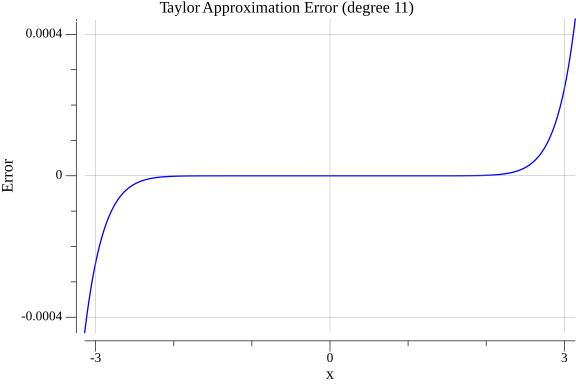
\includegraphics[width=1.0\linewidth]{material/sin/taylor/sin_taylor_err_n05.png}
  \end{minipage}
\end{figure}

\begin{figure}[H]
  \centering
  \caption{$f(x) = \sin(x)$のテイラー展開（23次多項式）}
  \label{fig:sin-taylor-last}
  \vspace{5pt}
  \begin{minipage}[b]{0.48\linewidth}
    \centering
    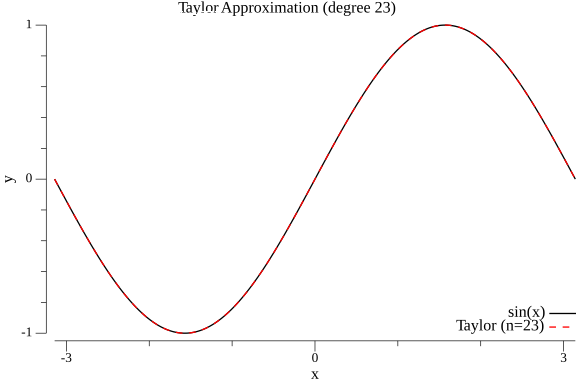
\includegraphics[width=1.0\linewidth]{material/sin/taylor/sin_taylor_n11.png}
  \end{minipage}
  \hfill
  \begin{minipage}[b]{0.48\linewidth}
    \centering
    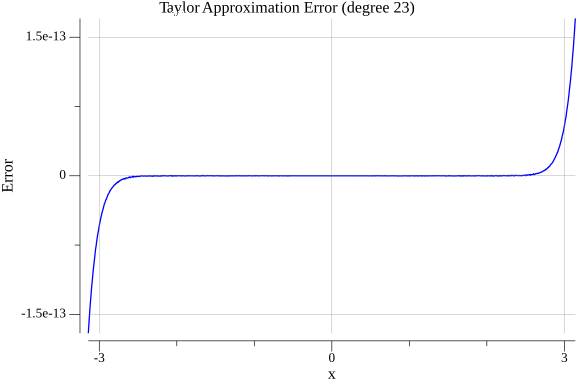
\includegraphics[width=1.0\linewidth]{material/sin/taylor/sin_taylor_err_n11.png}
  \end{minipage}
\end{figure}

